% !TEX root = ../thesis.tex
% !TEX spellcheck = en-US

\clearpage

\section{Methods}
\label{sec:Methods}

Text classification and related problems have been of interest for research for decades now as mentioned in the \nameref{sub:Related work} section (\ref{sub:Related work}). Therefore numerous approaches have been proposed to tackle this task. This section introduces the reader to two general types of approaches: First the method of using Vector Space Models for classification where each text is represented as a vector through transformations of the data and second the technique of modeling text as a sequence and applying algorithms that are specifically well-suited for learning temporal patterns of sequential signals.

This section will get be slightly more technical than the previous ones where needed to formally describe the techniques. Thus familiarity with fundamental concepts from Machine Learning, Function Approximation and Optimization, Probability Theory, Information and Decision Theory and a general knowledge of Linear Algebra is assumed. However all approaches are also introduced to some degree on a conceptual and intuitional level so that the basic ideas can be understood without this knowledge. The technically inclined reader on the other hand is encouraged to follow the suggested references on the techniques for further study and in-depth coverage that was beyond the scope of this work.

\subsection{Vector Space Models}
\label{sub:Vector Space Models}

Vector Space Models are a popular approach of modeling real world objects in a way that expresses their characteristics and structure through a numerical representation. Specifically we this representation assigns real-valued fixed-size vectors to each object, i.e. to each text document in the context of text classification. This means that our objects inhibit populate a common vector space $\mathcal{V}$.

To be a meaningful representation of data that let's us learn patterns this vector space $\mathcal{V}$ follows the contiguity hypothesis: \textquote{Documents in the same class form a contiguous region and regions of different classes do not overlap.}~\cite[Chapter 14, p.~289]{Manning:2008aa}. This means the similarity of objects is expressed through it's distance in the vector space. Further we often assume that the dimensions of a vector encode certain properties or latent factors of the objects or data we are modeling. This adds the notion of sub-vector distance where objects can be close and thus similar to each other with respect to only certain dimensions in the vector space, a property that encodes more fine-grained structure in the data and can be exploited by classification algorithms.

A concrete example for illustration is the Unigram model, the simplest form of N-Gram models which will be introduced in the next section: Each vector encodes word frequencies of words in an associated document, i.e. the vector is basically just a histogram of the word counts in this document. Looking at the histograms for several documents through can already visually reveal certain properties, such as topics if for instance lots of words regarding politics accumulate in one document whereas another document shows high frequencies of sports related terms.

The next sections will introduce two model approaches of this type with their properties and common variations. First N-gram models will be described that were already mentioned before and are in their core based on word (co-)occurrence frequencies. Then a more recent approach from the field of \gls{Representation Learning} will be discussed where word and document representations are automatically learned based through context prediction.

\subsubsection{N-gram Models}
\label{subs:N-gram Models (Methods)}

N-gram language models are based on co-occurrences of word or character sequences, so-called N-grams or $k$-shingles as they are referred to in the Data Mining literature~\cite[Chapter 3.2, p.~72]{Leskovec:2014aa}. Formally an N-gram is defined as a sequence of $n$ items, each of which consist of $n$ characters or words, effectively used to capture sub-sequences of text. Common choices are N-grams of size 1, 2 or 3 --- called \emph{unigrams}, \emph{bigrams} and \emph{trigrams} respectively --- and the definition can be extended to using a window size $[\textit{w}_{\text{min}}, \textit{w}_{\text{max}}]$, employing all combinations of N-grams in this interval.

N-grams are usually used to create a vector-space model by representing each document in a dataset as a \textit{bag-of-words} or \textit{bag-of-N-grams} vector so that each dimension of the vector represents statistics about the corresponding N-gram. Specifically, a common way to compute the word count vectors for a document is the following:

\begin{equation}
  \text{TF}_{ij} = \frac{f_{ij}}{\max_k f_{kj}}
\end{equation}

Where $f_{ij}$ is \textquote{the \emph{frequency} (number of occurences) of a term (word) $i$ in document $j$} and $\text{TF}_{if}$ is the \emph{term frequency}, i.e.   \textquote{$f_{ij}$ normalized by dividing it by the maximum number of occurrences of any term [\ldots] in the same document}~\cite[Chapter 1.3.1, p.~8]{Leskovec:2014aa}.

As this approach has been studied for decades there is quite an extensive amount of variants and thus hyper-parameters to tune. The most important ones will be explained in the following sections:

\paragraph{Words vs. Characters} The first choice when building an N-gram language model is to use characters or words as the atomic unit. In practically every case there are less characters than words in a dataset, but to capture expressive substrings usually larger N-gram window sizes or ranges have to be chosen, which leads to a combinatorial explosion. In case of word-based models on the other hand the maximal size of the feature space is the size of the vocabulary $\mathcal{V}$ in the case of unigrams or $V^k$ in case of $k$-grams.
par
\paragraph{Stop words}
\label{par:Stop words}
For creating N-gram models, so-called stop word lists are often used which are lists of frequent words that will be excluded as they do not carry much meaning~\cite[Chapter 1.3.1, p.~7]{Leskovec:2014aa}. The stop-word list used in these experiments is the standard list used for the Scikit-learn framework~\cite{Pedregosa:2011aa} is made available by the University of Glasgow Information Retrieval group\footnote{\url{http://www.gla.ac.uk/schools/computing/research/researchoverview/informationretrieval/}. The full stop word list can be found in the Appendix in Section~\ref{sub:Stopwords for N-grams}.}.

\paragraph{N-gram range} The N-gram range, also known as window size or shingle size, refers to combinations of the atomic units of the model (words or characters) and defines an upper and lower limit for these combinations. For example a range of $[1,1]$ specifies a unigram model, $[2,2]$ a bigram model and $[1,2]$ a combination of both including all unigrams and all bigrams.
A larger range allows the model to capture an increasing amount of word order and thus context, but again leads to a combinatorial explosion in terms of feature space.

\paragraph{Vector size} The vector size imposes an upper limit to the vector size and therefor the number of N-grams that can be encoded in the feature space. Commonly this simply uses the words with the highest frequency to reduce the vector size from the full length --- the size of the vocabulary --- to the desired size.

\paragraph{TF.IDF weighting}
\label{par:TF.IDF weighting}
A common extension to using word-counts is to weight the term frequencies by the so-called inverse document frequency, i.e.\ the inverse of the frequency of an term or N-gram in all documents. This method is commonly referred to as \emph{TF.IDF} and specifically the inverse document frequency is defined as $\text{IDF}_i = \log_2 (N/n_i)$, where logarithmic smoothing is applied. The TF.IDF value for a term or N-gram is then computed as $\text{TF}_{ij} \cdot \text{IDF}_i$.

\paragraph{Sublinear TF scaling}
\label{par:Sublinear TF scaling}
 As~\cite[Chapter 6.4.1, p.~126]{Manning:2008aa} suggests \textquote{[it] seems unlikely that twenty occurrences of a term in a document truly carry twenty times the significance of a single occurrence}. Hence a common variant is \emph{sublinear scaling} where we down-weigh the increase in term importance by applying a logarithmic function to it, resulting in the sub-linear term frequency $\text{subTF}_{ij}$:

\begin{displaymath}
  \text{subTF}_{ij} = \left \{ \begin{array}{l l} 1+\log \text{TF}_{ij} & \text{TF}_{ij} > 0 \\
  0 & \text{otherwise}
\end{array} \right \}
\end{displaymath}

\paragraph{Normalization} Often the term vectors are globally normalized using the $L_1$ or $L_2$ norm to remove the effect of statistical differences between the terms.

There are, of course, various other variants and modifications to the N-gram model, but within the scope of this thesis only the most notable ones were introduced and will be used for experiments later. For further material on this subject refer for example to~\cite{Manning:2008aa}.

\bigskip

Today N-gram models are still in wide use and considered as state of the art \textquote{not because there are no better techniques, but because those better techniques are computationally much more complex, and provide just marginal improvements}~\cite[p.~17]{Mikolov:2012aa}. As~\cite{Mikolov:2012aa} points out further \textquote{[the] most important weakness is that the number of possible n-grams increases exponentially with the length of the context, preventing these models to effectively capture longer context patterns. This is especially painful if large amounts of training data are available, as much of the patterns from the training data cannot be effectively represented by n-grams and cannot be thus discovered during training. The idea of using neural network based LMs [Language Models] is based on this observation, and tries to overcome the exponential increase of parameters by sharing parameters among similar events, no longer requiring exact match of the history H.}~\cite[p.~17]{Mikolov:2012aa}

\subsubsection{Distributed Continuous Representations}
\label{subs:Distributed Continuous Representations}

\begin{wrapfigure}{h!}{0.5\textwidth}
  \begin{center}
    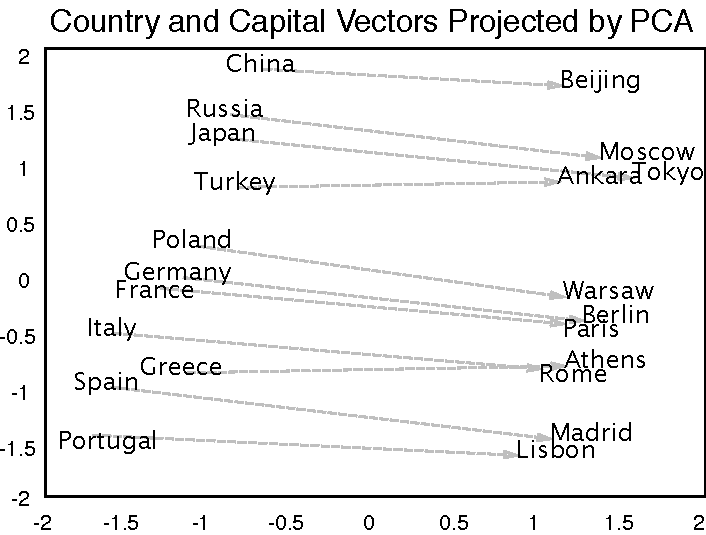
\includegraphics[width=0.48\textwidth]{img/word2vec_cities.pdf}
  \end{center}
  \caption{Two-dimensional PCA projection of the 1000-dimensional Skip-gram vectors of countries and their capital cities. (Adapted from~\cite{Mikolov:2013ac})}
\label{fig:word2vec-cities}
\end{wrapfigure}

To overcome the shortcomings of popular language models such as the ones of the N-gram model mentioned above, lots of recent work went into the study of so-called distributed language models. One branch of research that gained significant attention is the work on Neural Network based Language models (NNLMs), popularized largely through the work of T. Mikolov and his software realization of such a model dubbed \emph{word2vec} with interest coming not only from the academic community.

His work builds on ideas introduced in~\cite{Bengio:2000aa} where a neural network based model was proposed for modeling high-dimensional discrete data, which was then applied to the domain of language modeling in~\cite{bengio2003neural} and the idea of learned distributed representations goes back to~\cite{Hinton:1986aa}. Following the description in~\cite{Bengio:2000aa}, the approach is as follows:

\begin{enumerate}
  \item Associate with each word in the vocabulary a distributed \emph{word feature vector} (a real-valued vector in $\mathbb{R}^m$),
  \item Express the joint \emph{probability function} of word sequences in terms of the feature vectors of these words in the sequence, and
  \item Learn simultaneously the \emph{word feature vectors} and the parameters of that \emph{probability function}.
\end{enumerate}

To achieve this, a feedforward neural network model is trained to learn these \emph{word feature vectors} or \emph{word embeddings}. As input a sequence of $n$ words is given, each encoded using one-hot encoding or one-of-$V$ encoding where the corresponding indicator vectors for each word have the size of the vocabulary $V$. The input word vectors are then projected linearly into a projection layer of significantly lower dimensionality $D$, using a global projection matrix for across all words, and concatenated, forming the input of size $D \times N$ to a hidden layer of size $H$. The hidden layer then feeds non-linearly into the output layer that is again of size $V$, modeling the probability distribution for a word given its context $P(w_t \mid w_{t - n}, \ldots, w_{t - 2}, w_{t - 1})$.

\paragraph{Simplified Continuous Models}

\cite{Mikolov:2013ad} then introduced two simplified models, removing the hidden layer and only using a projection layer, with shared weights for all words. The Continuous Bag-of-Words Model (CBOW) model is trained to predict the current word $w_t$ given the $k$ words around it. Its name is due to the fact that the word order does not influence the projection as the word vectors are summed or averaged. The Continuous Skip-gram Model works the other way around, predicting the most likely $k$ words around a given word $w_t$. Figure~\ref{fig:cbow-skip-gram} illustrates both models.


\begin{figure}[h]
    \centering
    \begin{subfigure}[b]{0.49\textwidth}
        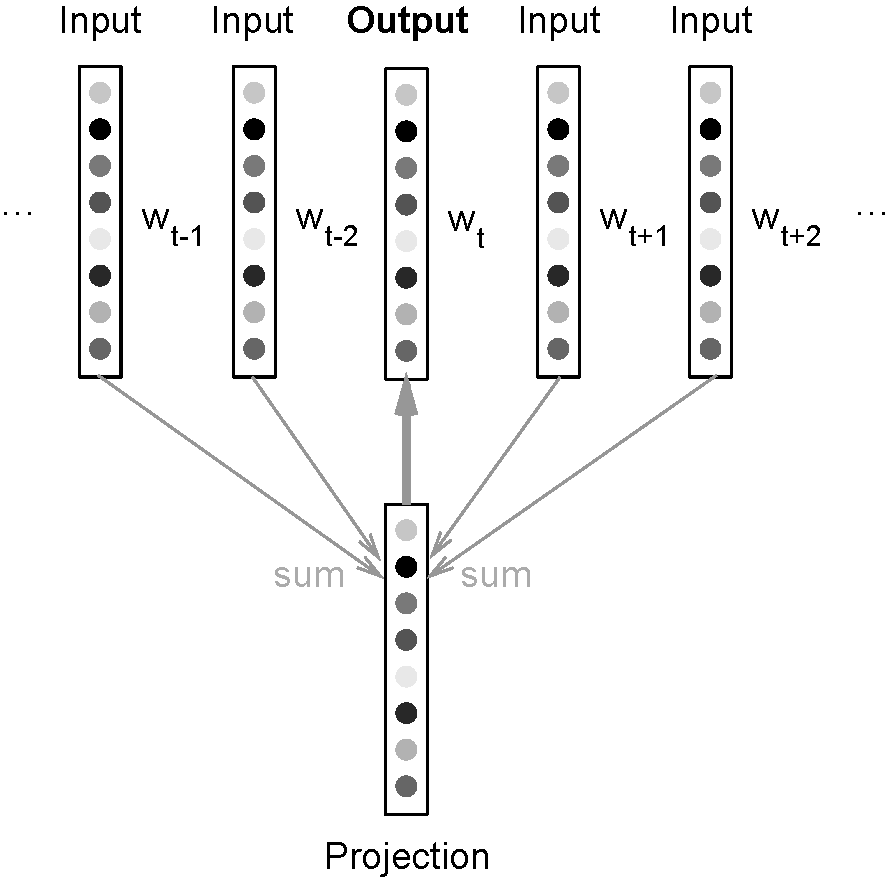
\includegraphics[width=\textwidth]{img/cbow_vert2.pdf}
        \caption{Continuous Bag-of-Words Model}
\label{fig:cbow}
    \end{subfigure}
    %add desired spacing between images, e. g. ~, \quad, \qquad, \hfill etc.
      %(or a blank line to force the subfigure onto a new line)
    \begin{subfigure}[b]{0.49\textwidth}
        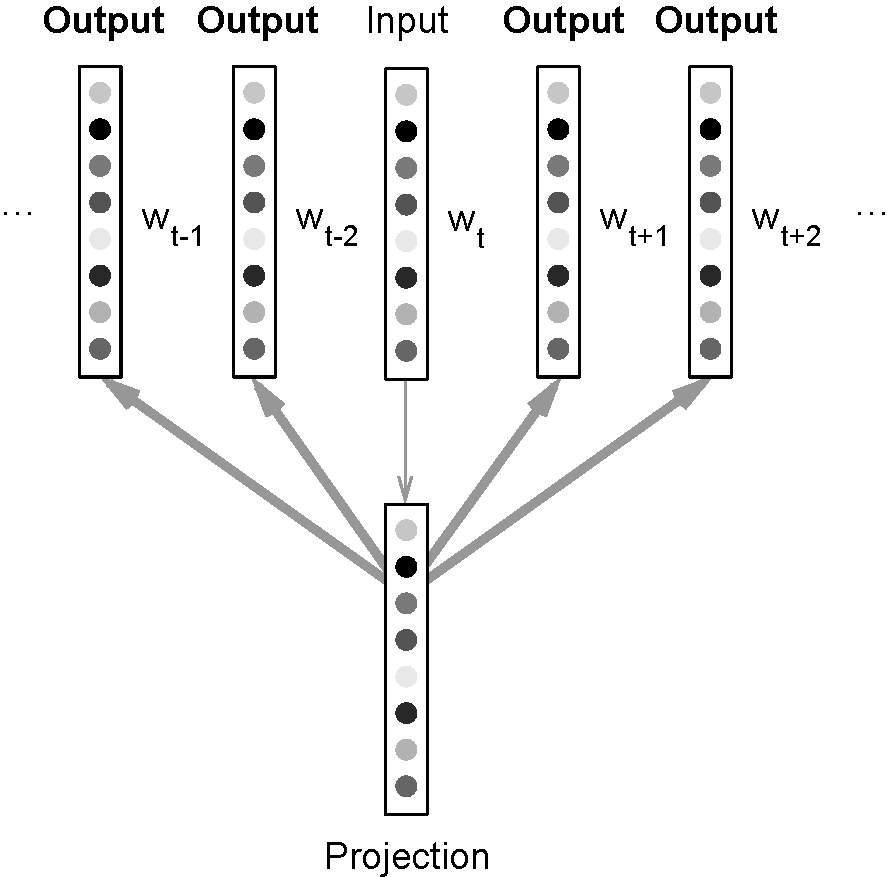
\includegraphics[width=\textwidth]{img/skip-gram_vert2.pdf}
        \caption{Continuous Skip-gram Model}
\label{fig:skip-gram}
    \end{subfigure}
    \caption{Architectures for learning continouus distributed word vectors, adapted from~\cite{Mikolov:2013ad}}
\label{fig:cbow-skip-gram}
\end{figure}

These models have been shown to outperform state of the art N-gram models on various tasks (see e.g.~\cite{bengio2003neural} or~\cite{Mikolov:2012aa}). An interesting outcome of this research is the fact that these \emph{word vectors} capture many interesting and often subtle semantic regularities and that these can be exploited explicitly in an algebraic manner. When trained on an extensive dataset, one can perform calculations as $v(Paris) - v(France) + v(Germany)$ and the closest vector to the result turns out to be $v(Berlin)$ where $v(\cdot)$ denotes the \emph{word vector} of a word. Figure~\ref{fig:word2vec-cities} shows a PCA projection of Skip-gram trained vectors of countries and their capital cities.


A notable alternative to these models was developed by~\cite{Pennington:2014aa}. In their model called \emph{GloVe}, which stands for global vectors, they construct a vector space model with similar properties as the models introduced above, which instead relies global word-word co-occurrence counts. This method thus operates directly in the co-occurrence statistics of the corpus compared to the Neural Network based methods that \textquote{fail[\ldots] to take advantage of the vast amount of repetition in the data}~\cite{Pennington:2014aa}.


There have been various extensions and variants to the Neural Network based language models especially, including architectures based on Recurrent Neural Networks (see~\cite{Mikolov:2012aa}). Some of the most important variations will are discussed in the following section as they were evaluated in the experiments:

\subparagraph{Hierarchical Softmax}
The architectures proposed in~\cite{Bengio:2000aa},~\cite{bengio2003neural} and follow-up work use a \emph{softmax} activation function at the output layer in order to obtain valid probabilities for each word to be predicted:

\begin{equation}
  \operatorname{softmax}(\mathbf{x}_j) = \frac{\exp(\mathbf{x}_j)}{\sum_k \exp(\mathbf{x}_k)}
\end{equation}

\emph{Hierarchical Softmax} uses a binary tree to encode the output which leads to an efficient approximation of the full softmax and speeds up training and inference. Details can be found in~\cite{Mikolov:2013ab}.

\subparagraph{Negative Sampling}
Another technique applied by~\cite{Mikolov:2013ab} \emph{Negative Sampling} which is a simplified version of Noise Contrastive Estimation (NCE) introduced by~\cite{Gutmann:2012aa}. Based on the insight that a good model should be able separate noise from signal, this method mixes samples from a noise distribution into the signal to be learned, in this case random words that are not in the context window, which is shown to approximately maximize the log probability of the softmax. Free parameters of this technique are the number of negative samples $k$ per data sample and the noise distribution $P_n(w)$

\subparagraph{Sub-sampling of Frequent Words}
As there the difference between frequent and infrequent words in large corpora can be huge and the frequent words often don't carry as much meaning, in~\cite{Mikolov:2013ab} a simple sub-sampling technique is used to counter this imbalance by discarding words with a probability computed as follows:

\begin{equation}
  P(w_i) = 1 - \sqrt{\frac{t}{f(w_f)}}
\end{equation}

with $f(w_i)$ denoting the frequency of word $w_i$ and $t$ denoting a threshold. \cite{Mikolov:2013ab} state that this method, while chosen heuristically, \textquote{accelerates learning and even significantly improves the accuracy of the learned vectors of the rare words}.

\subsubsection*{Distributed representations for documents}
\label{subs:Distributed representations for documents}

The models explained above are defined on words as the atomic unit. Therefore several ways have been proposed to extend these to sequences of words in order to obtain a vector space of sentences or documents. A few of these will be briefly outlined here:

\subparagraph{Compositional Models and Bag-of-Means}
\label{subp:Bag-of-Means}

Several approaches of composing document vectors out of word vectors have been studied in \cite{Mitchell:2010aa}. One of the most successful variants evaluated was weighted averaging of word embeddings, a technique also referred to as \emph{Bag-of-Means}. However this approach \textquote{loses the word order in the same way as the standard bag-of-words models do.}~\cite{Le:2014aa}. This intuitive property was confirmed by~\cite{Zhang:2015aa} where the method consistently performed poorest in comparison to other approaches on a variety on tasks.

\subparagraph{Paragraph Vectors}
\label{subp:Paragraph Vectors}

In~\cite{Le:2014aa} a different approach is shown that builds on the same idea as the original word2vec model. In particular two approaches proposed. The first model, dubbed \emph{Distributed Memory (PV-DM)} is similar to the continuous Bag-of-Words model as a word is predicted given the words in the context, but additionally a paragraph token is used as an input to the model. To the algorithm this simply acts as another word index but it identifies the paragraph the words stem from and serves as a context memory for this paragraph.
The second approach is called \emph{Distributed Bag-Of-Words (PV-DBOW)} and does not use word prediction at all. Instead words are sampled from a paragraph and the associated paragraph vector has to be learned to predict these words as well as possible. This model is therefore more similar to the Skip-Gram model by~\cite{Mikolov:2013a} as the several words are predicted using a single learned representation. At inference time both models need to construct new Paragraph Vectors for unseen paragraphs using a slightly varied learning procedure (see~\cite{Le:2014aa}).

\subsection{Methods For Classification With Vector Space Models}
\label{sub:Methods For Classification With Vector Space Models}

Many classical machine learning algorithms work on data in a fixed-dimensional vector format and can thus be applied to a vector space model as described in the previous section. Here a set of well-known algorithms will be briefly introduced, each representing a family of approaches with different model assumptions. It should be pointed out that there exist a plethora of other models and algorithms that can be used, the ones chosen here though are widely considered standard methods and have proven successfully in the past for a wide range of problems.

% \paragraph{Classification Schemes}
% \label{par:Classification Schemes}
% There are three common schemes for classification: In \emph{binary classification} there is only a single class and for each document we decide whether or not it belongs to this class. A classic example is email spam detection where we predict if a given email is spam or not. \emph{Multi-class classification} assumes the existence of more than one class and can be sub-categorized into \emph{single-label classification} where the labels are mutually exclusive and and \emph{multi-label classificaion} where they are not and thus multiple labels can be assigned to a single document at the same time. These settings also need be evaluated differently which will be discussed in Section~\ref{sub:Evaluation}.




% A simple approach to multi-class classification is to pose the learning problem as a combination of binary classification problems as described in~\cite[Chapter 4.1.2, p.~182]{Bishop:2006aa}. This can be done by using $K$ separate classifiers, each of which predicts one of the classes against all $K-1$ other classes, which is known as the \textit{one-versus-the-rest} classification scheme. An alternative approach is to train $K (K - 1) / 2$ binary classifiers for each possible pair of classes, referred to as \textit{one-versus-one} classification.
%
% These extensions though have major drawbacks as pointed out by~\cite[Chapter 5.2.2]{Duda:1973aa}. As illustrated by~\ref{fig:Bishop2006aa-p182-ch4-fig4-1} both of the classification schemes lead to ambiguous regions in the hypothesis space as their classification is undefined.
%
% \begin{figure}[h]
%     \centering
%     \begin{subfigure}[b]{0.4\textwidth}
%         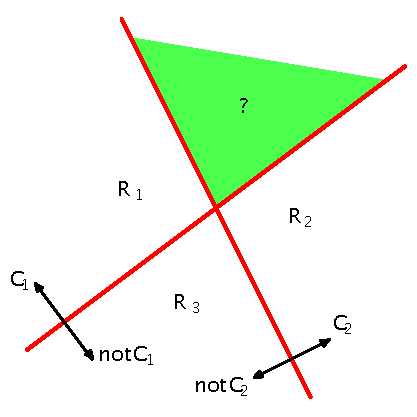
\includegraphics[width=\textwidth]{img/Bishop2006aa-p182-ch4-fig4-1-a.pdf}
%         \caption{One-Vs-Rest classification scheme}
%         \label{fig:Bishop2006aa-p182-ch4-fig4-1-a}
%     \end{subfigure}
%     ~ %add desired spacing between images, e. g. ~, \quad, \qquad, \hfill etc.
%       %(or a blank line to force the subfigure onto a new line)
%     \begin{subfigure}[b]{0.4\textwidth}
%         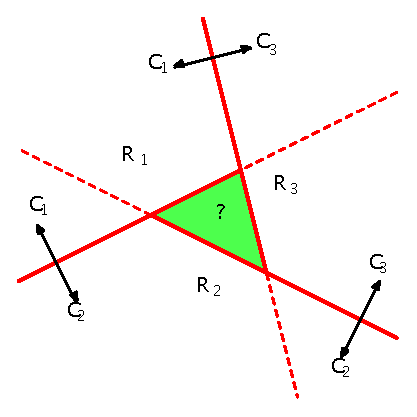
\includegraphics[width=\textwidth]{img/Bishop2006aa-p182-ch4-fig4-1-b.pdf}
%         \caption{One-Vs-One classification scheme}
%         \label{fig:Bishop2006aa-p182-ch4-fig4-1-b}
%     \end{subfigure}
%     \caption{: Ambiguous regions in the hypothesis space (\cite{Bishop:2006aa} Chapter 4, Figure 4.1) }
%     \label{fig:Bishop2006aa-p182-ch4-fig4-1}
% \end{figure}

\subsubsection{Generalized Linear Models}
\label{subs:Generalized Linear Modelsl}

Generalized Linear Models are an extension of linear discriminant functions. Whereas discriminant functions and ordinary linear regression models produce linear decision boundaries in the input space (\emph{linear-response model}), Generalized Linear Models apply a non-linear \emph{link function} or \emph{basis function} to the input, making it possible for the model to achieve non-linear decision boundaries in the original input space while corresponding to a linear decision boundary in the feature space.

The most prominent algorithm in this class is \emph{Logistic Regression} which uses the \emph{logistic sigmoid} function as a basis function:

\begin{equation}
  \sigma (a) = \frac{1}{1 + \exp(-a)}
  \label{eq:sigmoid}
\end{equation}

This yields posterior class probabilities of:

\begin{equation}
  p(\mathcal{C}_n \mid \phi) = y(\phi) = \sigma(w^T  \phi)
\end{equation}

where $w$ is the learned \emph{weight vector} with the free parameters of the model, $\phi$ is the \emph{feature vector} of inputs transformed through the basis function $\sigma$ and $y$ is the model function that we use to infer class predictions from our data.

Using a the maximum likelihood method we can now find a set of parameters for our model function $y$ that gives us the predictions with the lowest error. For a dataset $\{ \phi_n, t_n \}$, where $t_m \in {0, 1}$ and $\phi_n = \phi(x_n)$, with $n = 1, . . ., N$ denoting the amount of data points:

\begin{equation}
  p(\mathbf{t} | w) = \prod_{n=1}^N y_n^{t_n} \{ 1 - y_n \}^{1-t_n}
\end{equation}

where $\mathbf{t} = (t_1, \ldots, t_N)^T$ and $y_n = p(\mathcal{C}_n \mid \phi)$. We can now define an error function by taking the negative logatirhm of the likelihood, which is called the \emph{cross-entropy} error function:

\begin{equation}
  E(\mathbf(w)) = - \ln p(\mathbf{t} | w) = - \sum_{n=1}^N \{ t_n \ln y_n + (1 - t_n) \ln (1-y_n) \}
\end{equation}

where $y_n = \sigma(a_n)$ and $a_n = \mathbf{w}^T \phi_n$. When taking the gradient we with resepect to $\mathbf{w}$ we obtain:

\begin{equation}
  \nabla E(\mathbf{w}) = \sum_{n=1}^N (y_n - t_n) \phi_n
\end{equation}

From here we can apply an optimization procedure such as gradient descent to arrive at a weight vector $\mathbf{w}$ that minimizes the error function above. A deeper treatment of the Logistic Regression and Generalized Linear Models can be found in many introductory textbooks such as~\cite[Chapter 4.3.2, p.~205]{Bishop:2006aa}.

\todo{mention one-vs-all and multinomial}

\subsubsection{Bayesian Classifiers}
\label{subs:Bayesian Classifiers}

Bayesian Classifiers are a family of probabilistic models derived from Bayes' Theorem, which itself is a simple application of the rule conditional probability:

\begin{equation}
  p(A \mid B) = \frac{P(B \mid A) P(A)}{P(B)}
\end{equation}

Where $P(A)$ is the probability of A and $P(A \mid B)$ conditional probability of A given B. In the Bayesian interpretation probabilities represent a degree of belief that changes under the observation of evidence. The following form is usually referred to as Bayes' rule and expresses this interpretation:

\begin{equation}
  \underbrace{p(A \mid B)}_{posterior}  \propto \underbrace{P(B \mid A)}_{likelihood} \underbrace{P(A)}_{prior}
\end{equation}

where $P(B)$ is marginalized out as a normalization constant of the probabilities. This simple rule forms the basis of a whole subfield of Bayesian Inference (see e.g.\ the textbook~\cite{Barber:2012aa} for a good coverage of the topic).

The most known Bayesian classification algorithm is the \emph{Naive Bayes} classifier, a simple class-conditional generative model which builds on the assumption that all data points are conditionally independent given the classes $\mathcal{C}_n$. For each class $c_j$ we can predict it's probability given an input vector $\mathbf{x}$ as:

\begin{equation}
  p(\mathbf{x}) = p(c_j) \prod_{i=D}^D p(x_i \mid c_j)
\end{equation}

We can then use Bayes' rule to form a classifier for each class:

\begin{equation}
  p(c_j \mid \mathbf{x}) = \frac{p(\mathbf{x} \mid c_j ) p(c_j)}{ p (\mathbf{x})} = \frac{p(\mathbf{x} \mid c_j ) p(c_j)}{ \sum_c p(\mathbf{x \mid c} p(c)) }
\end{equation}

We can then choose the class with the highest class probability as our prediction. Again there are numerous variants and related models to Naive Bayes and it can be regarded as a simple \emph{graphical model}, a family of techniques which are covered e.g.\ in~\cite{Barber:2012aa} or~\cite{Bishop:2006aa}.

\todo{more on ML estimation?}

\subsubsection{Tree Based Methods}
\label{subs:Tree Based Methods}

\begin{wrapfigure}{r}{0.5\textwidth}
  \centering
  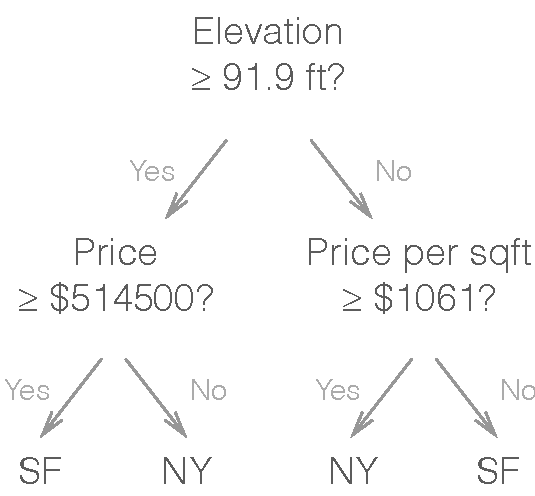
\includegraphics[width=0.48\textwidth]{img/decision-tree.pdf}
  \caption{A simple Decision Tree to determine whether a building is located in New York (NY) or San Francisco (SF).}
\label{fig:decision-tree}
\end{wrapfigure}

A simple but widely used classification as well as regression method are \emph{Decision Trees} which work by recursively partitioning the input space into dichotomous subregions, producing a binary decision tree. At inference time the resulting tree can then be used to produce an output by navigating through a path from its root to a leaf, answering a binary questions at each node to determine which child node to query next. Figure~\ref{fig:decision-tree} shows the visualization of an exemplified such a tree\footnote{Adapted from R2D3's ``visual introduction to Machine Learning'' at \url{http://www.r2d3.us/visual-intro-to-machine-learning-part-1/}}.
Every node represents a threshold in the input space that  the input data is compared against, corresponding to a decision such as ``Is the elevation of this building's elevation higher than or equal to 91.9 feet?''. If the answer is ``Yes'' the left child node is queried next, otherwise the right. This procedure is repeated until a leaf with a final answer is reached.

The technique was first introduced by~\cite{Breiman:1984ab} under the term \emph{Classification And Regression Tree (CART)} but exists in many variants. Learning such a model involves specifying the structure of the tree, including which input variable to query at each node in the graph and what each of the nodes' threshold values are. Since commonly it is computationally infeasible to generate and evaluate all possible decision trees for a given problem, a greedy procedure is usually chosen. We start with determining a first split in the data that represents the root node and grow the tree one node at a time, each node in the tree being determined by choosing splits that minimize an error measure.

Let $p_{\tau k}$ be the proportion of data points in region $R_{\tau}$ that are assigned to class $k$. Then we define the error as the negative cross-entropy:

\begin{equation}
  Q_{\tau}(T) = \sum_{k=1}^K p_{\tau k} \ln p_{\tau k}
\end{equation}

A common alternative for the classification error is the \emph{Gini index}:

\begin{equation}
  Q_{\tau}(T) = \sum_{k=1}^K p_{\tau k} (1 - p_{\tau k})
\end{equation}

Both measures vanish for $p_{\tau k} = 0$ and $p_{\tau k} = 1$ and are maximal at $p_{\tau k} = 0.5$, thus rewarding regions with a high proportion of data points assigned to one class. As~\cite[Chapter 14.4, p.~664]{Bishop:2006aa} notices \textquote{cross entropy and the Gini index are better measures than misclassification rate for growing the trees because they are more sensitive to the node probabilities. Also, unlike misclassification rate, they are differentiable and hence better suited to gradient based optimization methods}.

Decision trees are often chosen because they introduces next to no inductive model bias, but one has to be aware that this leads to high variance due to the Bias-Variance Dilemma. The algorithm is this prone to overfitting which is often countered by pruning, using a criterion that balances error with model complexity, such as:

\begin{equation}
  C(T) = \sum_{\tau=1}^{|T|} Q_{\tau}(T) + \lambda |T|
\end{equation}

Where $\lambda$ is a regularization parameter. Pruning of the tree happens after training a full tree as evidence shows that sometimes several splits occur that do not significantly reduce the error, followed by one that does~\cite[Chapter 14.4, p.~664]{Bishop:2006aa}.

\subsubsection{Ensemble Methods}
\label{subs:Ensemble Methods}

Another approach to machine learning algorithms are so-called \glspl{Ensemble Method}. These methods use different strategies to combine a set of classifiers, often employing techniques of \glspl{Randomized Algorithm}. There is a variety of such algorithms including \gls{Bagging}, \gls{Boosting} and \gls{Voting} methods which are covered in most of the popular introductory books to machine learning, e.g.~\cite{Bishop:2006aa}.

The Random Forests learning algorithm is a popular \gls{Ensemble Method} introduced by~\cite{Breiman:aa}. It is based on the concept of Decision Trees explained above, but instead of a single decision tree a set of trees, i.e.\ a forest, is grown on sets of bootstrapped samples from the input space. Specifically the algorithm grows $b = 1 \ldots B$ random trees by repeating the following steps for $b$ iterations:

\begin{enumerate}
  \item A \emph{bootstrapped sample} $S_i$ of data points is generated by drawing samples uniformly at random with replacement from the original data $D$. The sample is of smaller size than the dataset and is thus based on a subset of the input data. Notice that data can be sampled multiple times.
  \item A decision tree $T_i$ is trained on the bootstrapped data sample and is usually pruned at a certain limit of nodes.
\end{enumerate}

Then the resulting forest of trees ${T_1, \ldots, T_b}$ is used as an ensemble of classifiers using a majority vote over the predictions:

\begin{equation}
  C(X) = \frac{1}{B} \argmax_i \sum_{b = 1}^B \mathcal{I}(y_{T_b} = i)
\end{equation}

Where $\mathcal{I}(\cdot)$ is the indicator function. Other voting schemes have been proposed as well \todo{such as \ldots}.

\subsubsection{Instance-based Methods}
\label{subs:Instance-based Methods}

Another common class of learning algorithms are \emph{instance-based learning methods}, also known as \emph{example-based methods} or \emph{memory-based learning methods}. These methods directly use the given training examples and comparing new unseen examples with the training data at inference time, thus constructing the hypothesis directly from the data.

One of the most prominent instance-based classification methods is the \gls{kNN} algorithm which simply makes a class prediction based on the majority class amongst its $k$ nearest neighbors in the input space. This type of learning algorithm is a

The choice for the parameter $k$ depends on the type of problem and is often determined empirically via hyper-parameter optimization\todo{glossary?} or based on heuristics. The \gls{kNN} algorithm is highly prone to the curse of dimensionality as when a metric such as the Euclidean Distance is used as a metric for the \gls{kNN} algorithm to determine the nearest neighbors to the query vector there is little difference in the distance between samples in very high-dimensional spaces. Thus often \gls{Feature Extraction} or \gls{Dimensionality Reduction} techniques are employed before applying the \gls{kNN} algorithm.

\subsubsection{Kernel Methods}
\label{subs:Kernel Methods}

Kernel Methods are a set of instance-based methods (see Section~\ref{subs:Instance-based Methods}), as they construct the hypothesis and make predictions using the training data. Similar to other learning algorithms, kernel methods make use of transformations from an input space $\mathcal{X}$ into a another space $\mathcal{V}$. If the transformation is non-linear this allows a learning algorithm to learn a linear decision boundary in the projected space $\mathcal{V}$ which then corresponds to a non-linear decision boundary in the original space $\mathcal{X}$.

Kernel methods build on this idea and enable us to completely avoid the explicit mapping from the input space $\mathcal{X}$ to the transformed space $\mathcal{V}$ using the so-called \emph{kernel trick}: Using the fact that certain functions $k(x, x')$ in a space $\mathcal{X}$ can be expressed as an ianner product in another space $\mathcal{V}$, we can directly operate on the scalar dot products which can be interpreted as distances or similarities between the data. A function adhering to this property is called a \emph{kernel function} and a variety of such functions have been proposed, with extensions beyond transformations on real-valued vectors to kernel functions on complex objects such as graphs (see e.g.~\cite{Shervashidze:2011aa} for an interesting example of a graph kernel method).

A particularly successful classification method using kernels is the \gls{SVM} algorithm introduced by the name of \emph{Support Vector Networks} by~\cite{Cortes:aa}. Originally it was formulated as a linear classifier in~\cite{Vapnik:1982aa} and as such belongs to the family of generalized linear models introduced in Section~\ref{subs:Generalized Linear Modelsl}. This corresponds to using a so-called linear kernel as $k(x, y) = x^T y$. The \gls{SVM} belongs to the class of \emph{maximum margin classifiers}: Figuratively speaking and assuming linear separability and dichotomous classification, the decision boundary is trained to be maximally distant to the closest data points of each class. We can formalize the approach as follows:

We are given data points $x_1, \ldots, x_N$ and target values $t_1, \ldots, t_N$ for these points where $t_n \in {-1, 1}$ and $x_n \in \mathbb{R}^d$. We will use a linear model of the form:

\begin{equation}
	y(x) = w^T \phi(x) + b
	\label{eq:svm linear model}
\end{equation}

where $\phi$ denotes a transformation function. Then the perpendicular distance of a point $x$ to the decision hyperplane is given by

\begin{equation}
	\frac{|y(x)}{\|w\|}
\end{equation}

Since we want a hyperplane where all data points are correctly classified the decision boundary takes the form

\begin{equation}
	\frac{t_n y(x_n)}{\|w\|} = \frac{t_n (w^T \phi(x_n) + b)}{\|w\|}
\end{equation}

We now want to find the parameters $b$ and $w$ so that we maximize the margin which is given by the closest points to the decision boundary. This can be formulated as

\begin{equation}
	\argmax_{w, b} \left\{ \frac{1}{\|w\|} \min_n [ t_n (w^T \phi(x_n) + b) ] \right\}
\end{equation}

We can define the margin being one by scaling the input space which leads to the constraint that each point is either on the margin with distance 1 or further away:

\begin{equation}
	t_n (w^T \phi(x_n) + b) \geq 1 \quad\quad n = 1, \ldots, N
\end{equation}

We are thus given a constrained optimization problem which can be solved using Lagrange multipliers $a_n \geq 0$ giving:

\begin{equation}
	L(w, b, a) = \frac{1}{2} \|w\|^2 - \sum_{n=1}^N a_n \{ t_n (w^T \phi(x_n) + b) -1 \}
	\label{eq:svm lagrange}
\end{equation}

Taking the derivatives of $L$ with respect to $w$ and $b$ yields:

\begin{equation}
	w = \sum_{n=1}^N a_n t_n \phi(x_n)
	\label{eq:svm derivative w}
\end{equation}

\begin{equation}
	0 = \sum_{n=1}^N a_n t_n
	\label{eq:svm derivative b}
\end{equation}

Using Equations~\ref{eq:svm derivative w} and~\ref{eq:svm derivative b}, we can rewrite Equation~\ref{eq:svm lagrange} as:

\begin{equation}
	\widetilde{L}(a) = \sum_{n=1}^N a_n - \frac{1}{2} \sum_{n=1}^N \sum_{m=1}^N a_n a_m t_n t_m k(x_n, x_m)
\end{equation}

where $a$ is subject to the constrains

\begin{equation}
	a_n \geq 0 \quad \quad n = 1, \ldots, N
\end{equation}

\begin{equation}
	\sum_{n=1}^N a_n t_n = 0
\end{equation}

and the kernel function being defined as $k(x, x') = \phi(x)^T \phi(x')$.

Predictions on new data can then be made evaluating the sign in Equation~\ref{eq:svm linear model} where we can substitute $w$ using Equation~\ref{eq:svm derivative w}:

\begin{equation}
	y(x) = \sum_{n=1}^N a_n t_n k(x, x_n) + b
\end{equation}

Here due to the constraints for every data point either $a_n = 0$ or $t_n y(x_n) = 1$ so that all only points on the margin will remain in the sum and these are hence called \emph{support vectors}.

There are many extensions to the model with the most important one being the introduction of \emph{slack variables} by~\cite{Cortes:aa} in order to handle overlapping class distribution in the input space. Books dedicated to the topic such as~\cite{Shawe-Taylor:2004aa} offer a thorough introduction into Kernel Methods and again the topic is covered in most introductory books to machine learning.

\subsubsection{Neural Networks}
\label{subs:Neural Networks}

The \gls{NN} algorithm, often simply referred to as a \emph{Neural Network}, draws its inspiration and name form the way information processing in the brain is understood. Its biological analogy are neurons, nerve cells that can receive signals from other neurons through their input coannections called dendrites. A neuron can than react to this input by firing a signal to other neurons itself and this reacting depends on the strength of the incoming coannections which are adapted as an organism learns over time.

Modeling this behavior, a neural network is composed of multiple nodes, also referred to as \emph{neurons}. Each node can receive several signals from other nodes, combine these signals by applying an \emph{activation function} on their weighted sum and output a single signal as the result. The algorithm learns by adapting each single weight of this weighted sum for every node-to-node coannection.

\begin{figure}[h]
  \centering
  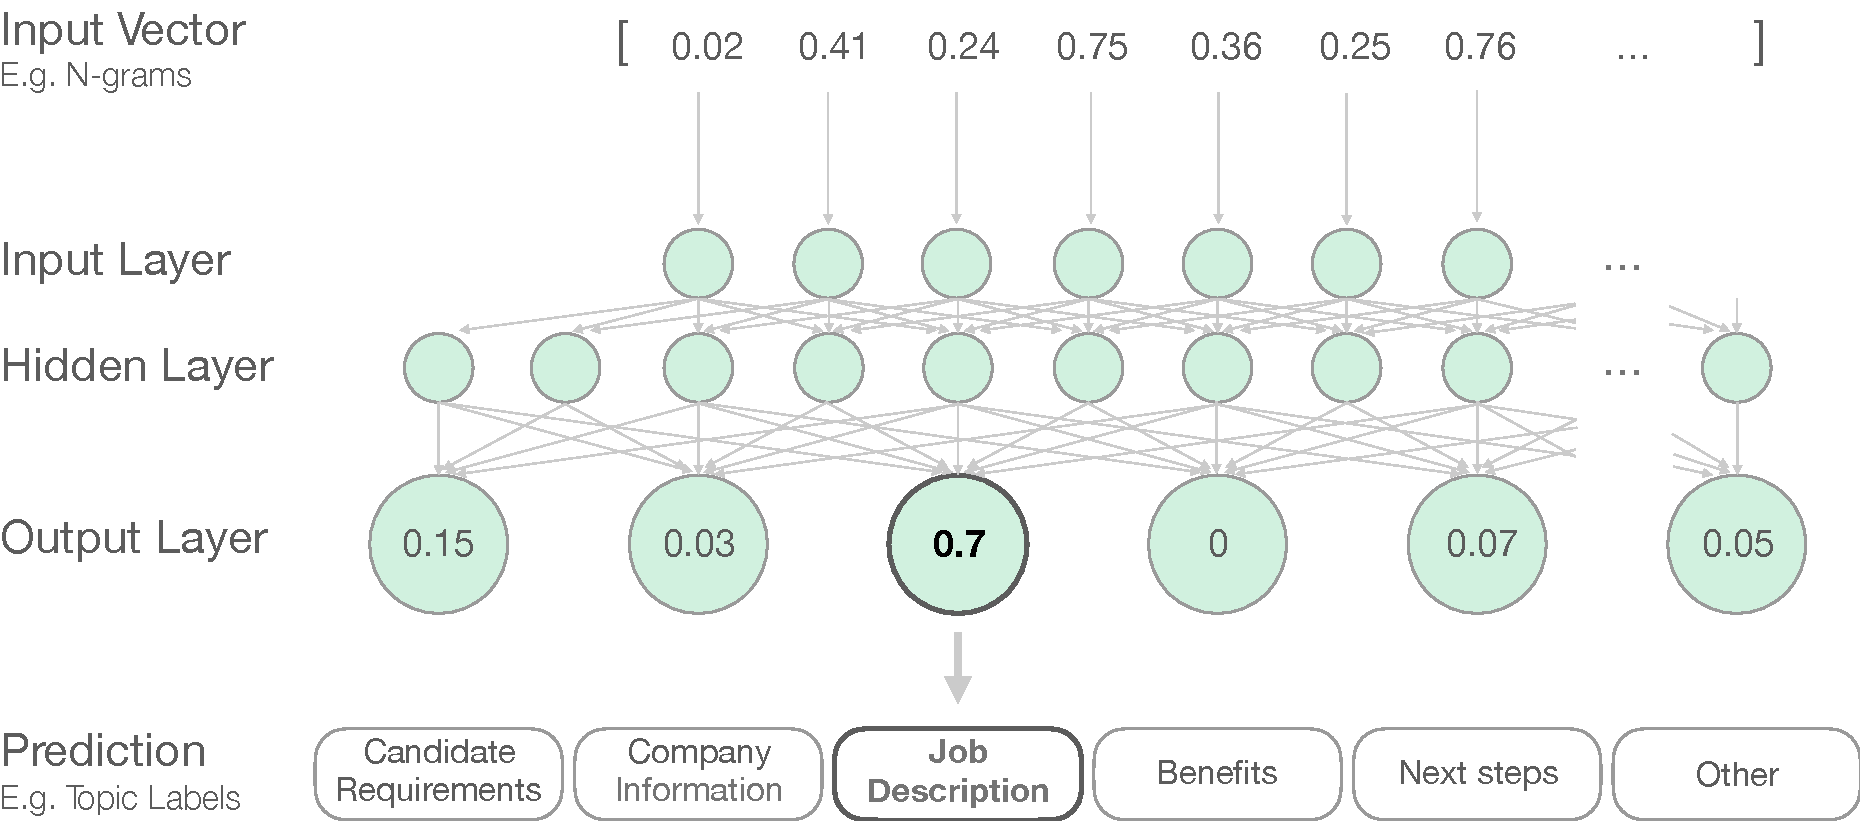
\includegraphics[width=1\textwidth]{img/NN}
  \caption{Conceptual visualization of a Feed-forward Neural Network}
  \label{fig:NN}
\end{figure}

The most common form, known as \emph{Feed-forward Neural Network}, is a network where all nodes of successive layers are coannected and each node in the network passes on its output signal to all nodes in the next layer until the transformed signal reaches the last layer. This layer represents the output signal or prediction and is thus called the \emph{output layer}. The first layer is called \emph{input layer} and is simply fed with real-valued vectors, e.g. as produced by a Vector Space method as described in Section~\ref{sub:Vector Space Models}. All layers in between are called \emph{hidden layers}. An exemplified illustration of such a feed-forward neural network with one hidden layer can be seen in Figure~\ref{fig:NN}.

For a single node the computation can formally be expressed as follows. We first compute the weighted sum of the inputs of the node:

\begin{equation}
  a_j = \sum_i w_{ji} z_i
  \label{eq:ann weighted sum}
\end{equation}

where $a_j$ is the weighted sum for node $j$, $w_kj$ is the weight for an input from node $i$ to node $j$ and $z_i$ is the output of node $i$. Then we apply the non-linear activation function $h(\cdot)$ to $a_j$ to receive the nodes output $z_j$:

\begin{equation}
  z_j = h(a_j)
  \label{eq:ann activation}
\end{equation}

For training the network it is essential that the activation function $h$ is differentiable. This is because we use partial derivatives of the error function with regards to each weight to obtain the error this weight is produced and update it accordingly. We can achieve this by making use of the chain rule for partial derivatives which, given the error in one layer, lets us derive the errors for the previous layer. This procedure is called \emph{backpropagation} since the error is propagated backwards through the network and will be described as follows.

First, using the chain rule, we can write the derivative of the error $E_n$ with respect to an incoming weight $w_{ji}$ as:

\begin{equation}
	\frac{\partial E_n}{\partial w_{ji}} = \frac{\partial E_n}{\partial a_j} \frac{\partial a_j}{\partial w_{ji}} = \delta_j z_i
	\label{eq:ann derivatives}
\end{equation}

where we use Equation~\ref{eq:ann weighted sum} and where $\delta_j$ denotes the \emph{error} at node $j$, defined as:

\begin{equation}
	\delta_j = \frac{\partial E_n}{\partial a_j}
	\label{eq:ann delta definition}
\end{equation}

Then for each output node $k$ given the sum-of-squares error we can directly calculate $\delta_k$ as follows:

\begin{equation}
	\delta_k = y_k - t_k
	\label{eq:ann output error}
\end{equation}

where $y_k$ denotes the computed output of node $k$ and $t_k$ the expected output, also called the \emph{target} value.

For hidden nodes we again apply the chain rule which yields

\begin{equation}
	\delta_j \equiv \frac{\partial E_n}{\partial a_j} = \sum_k \frac{\partial E_n}{\partial a_k} \frac{\partial a_k}{\partial a_j}
	= h'(a_j) \sum_k w_{kj}\delta_k
	\label{eq:ann backprop formula}
\end{equation}

by making use of Equations~\ref{eq:ann delta definition},~\ref{eq:ann weighted sum} and~\ref{eq:ann activation} and the fact that the error in node $j$ is a result of the errors in the nodes $k$ in the following layer in direction of the output.

Starting with the $\delta$ of the output nodes we can recursively apply Equation~\ref{eq:ann backprop formula} to compute all $\delta$'s in the network which then allows to compute the derivatives with regards to each weight using Equation~\ref{eq:ann derivatives}.

\begin{enumerate}
  \item We first perform a feed-forward pass, i.e. starting from the input nodes we propagate the signal through the network by successive application of weighted sum in Equation~\ref{eq:ann weighted sum} and  the activation function in Equation~\ref{eq:ann activation} until we receive output.
  \item Then we compute the $\delta_k$ of the error for each output node with Equation~\ref{eq:ann output error}.
	\item Next we can compute the $\delta$'s by backpropagating the errors using Equation~\ref{eq:ann backprop formula}.
	\item Lastly we can compute the derivatives for all weights using Equation~\ref{eq:ann derivatives} and adapt the weights by a learning rate to reduce the error.
\end{enumerate}

The study of Neural Networks comprises whole books and has been a subject of research for decades with strong fluctuations in popularity.
Recently there has been much interest in this technique again, especially regarding in Deep Neural Networks, i.e. networks with many hidden layers where the network can learn layers of data representations with increasing abstraction.
Various developments in research and technology, such as the available of massive parallel computational resources through \glspl{GPU} and learnings e.g.\ on the importance of initialization of the nodes in a network, have led to huge success in various application domains. Further there are various extensions to the learning procedure such as regularization methods and alternative network architectures such as the \gls{CNN}. It is beyond the scope of this work to cover these topics in depth and the interested reader shall be referred to any standard machine learning literature for an introduction to the topic, such as~\cite{Bishop:2006aa} from which this section's description was adapted. For a more recent treatment on the topic and on \gls{Deep Learning} in particular \cite{Bengio:2015aa} offers a great overview and  \cite{Cho:2014aa}
Various developments in research and technology, such as the available of massive parallel computational resources through \glspl{GPU} and learnings e.g.\ on the importance of initialization of the nodes in a network, have led to huge success in various application domains. Further there are various extensions to the learning procedure such as regularization methods and alternative network architectures such as the \gls{CNN}. It is beyond the scope of this work to cover these topics in depth and the interested reader shall be referred to standard machine learning literature for an introduction to the topic, such as~\cite{Bishop:2006aa} from which this section's description was adapted. For a more recent treatment on the topic and on \gls{Deep Learning} in particular \cite{Bengio:2015aa} offers a great overview and \cite{Cho:2014aa}, a Ph.D. thesis published at Aalto University two years ago, gives a broad coverage of the field as well.

\subsection{Sequential Models For Text Classification}
\label{sub:Sequential Models For Text Classification}

In Section~\ref{sub:Vector Space Models} we covered an approach to text classification where each text segment to be classified was first transformed into a fixed size vector representation and fed into a classifier afterwards. This approach treats each text segment as a document and assumes it belongs to a certain class.

An alternative approach is to model text as a sequential signal produced over time, similar to a time-series. This assumes strong dependencies between the current time step and previous time steps in the signal.
We can take this view with different levels of granularity: The most fine-grained representation of text are characters so text can just be seen as a sequence of characters, but also using words or sentences as the atomic unit would be possible. As the space of possible letters in most western languages is quite limited we can directly use these as states that our signal can take. In the case of words or longer sequences we would either have a huge space of states where similarity of words would be disregarded or we could use a vector space representations for words or sequences.

There are various algorithmic approaches to model time-series and sequences of evolving states such as Linear Dynamic Systems or Hidden Markov Models. However many of these methods tend to ``forget fast'', i.e. they are unable to model long-term dependencies. An extreme case are HMM's where the next state only depends on the current state. Here we will look at Recurrent Neural Networks in particular which are attractive for their ability to model long-term dependencies.

\subsubsection*{Recurrent Neural Networks}
\label{subs:Recurrent Neural Networks}

Recurrent Neural Networks are networks with loops, meaning that in contrast to Feedforward Neural Networks they can have coannections feedback coannections from a neuron's output back into it's input. This allows the network to pass information between time steps. Conceptually this can be thought of as a neural network copied $T$ times along the depth axis where the output of nodes $k_t$ at time step $t$ is coannected to the input of the same node in the successive copy $k_{t+1}$ at time step $t+1$. This process of turning a network with feedback loops into a three dimensional feedforward network with coannections between the time steps is called \emph{unrolling}.
It also provides a way for training the network where the standard back-propagation algorithm for Feedforward Neural Networks (see Section~\ref{subs:Neural Networks}) can be extended to incorporate these dependencies, then called \emph{Back-propagtion through time (BPTT)} introduced by~\cite{Werbos:1988aa} and others independently. A visualization of such an unrolled network for a single node is shown in Figure~\ref{fig:RNN}.

\begin{figure}[h]
  \centering
  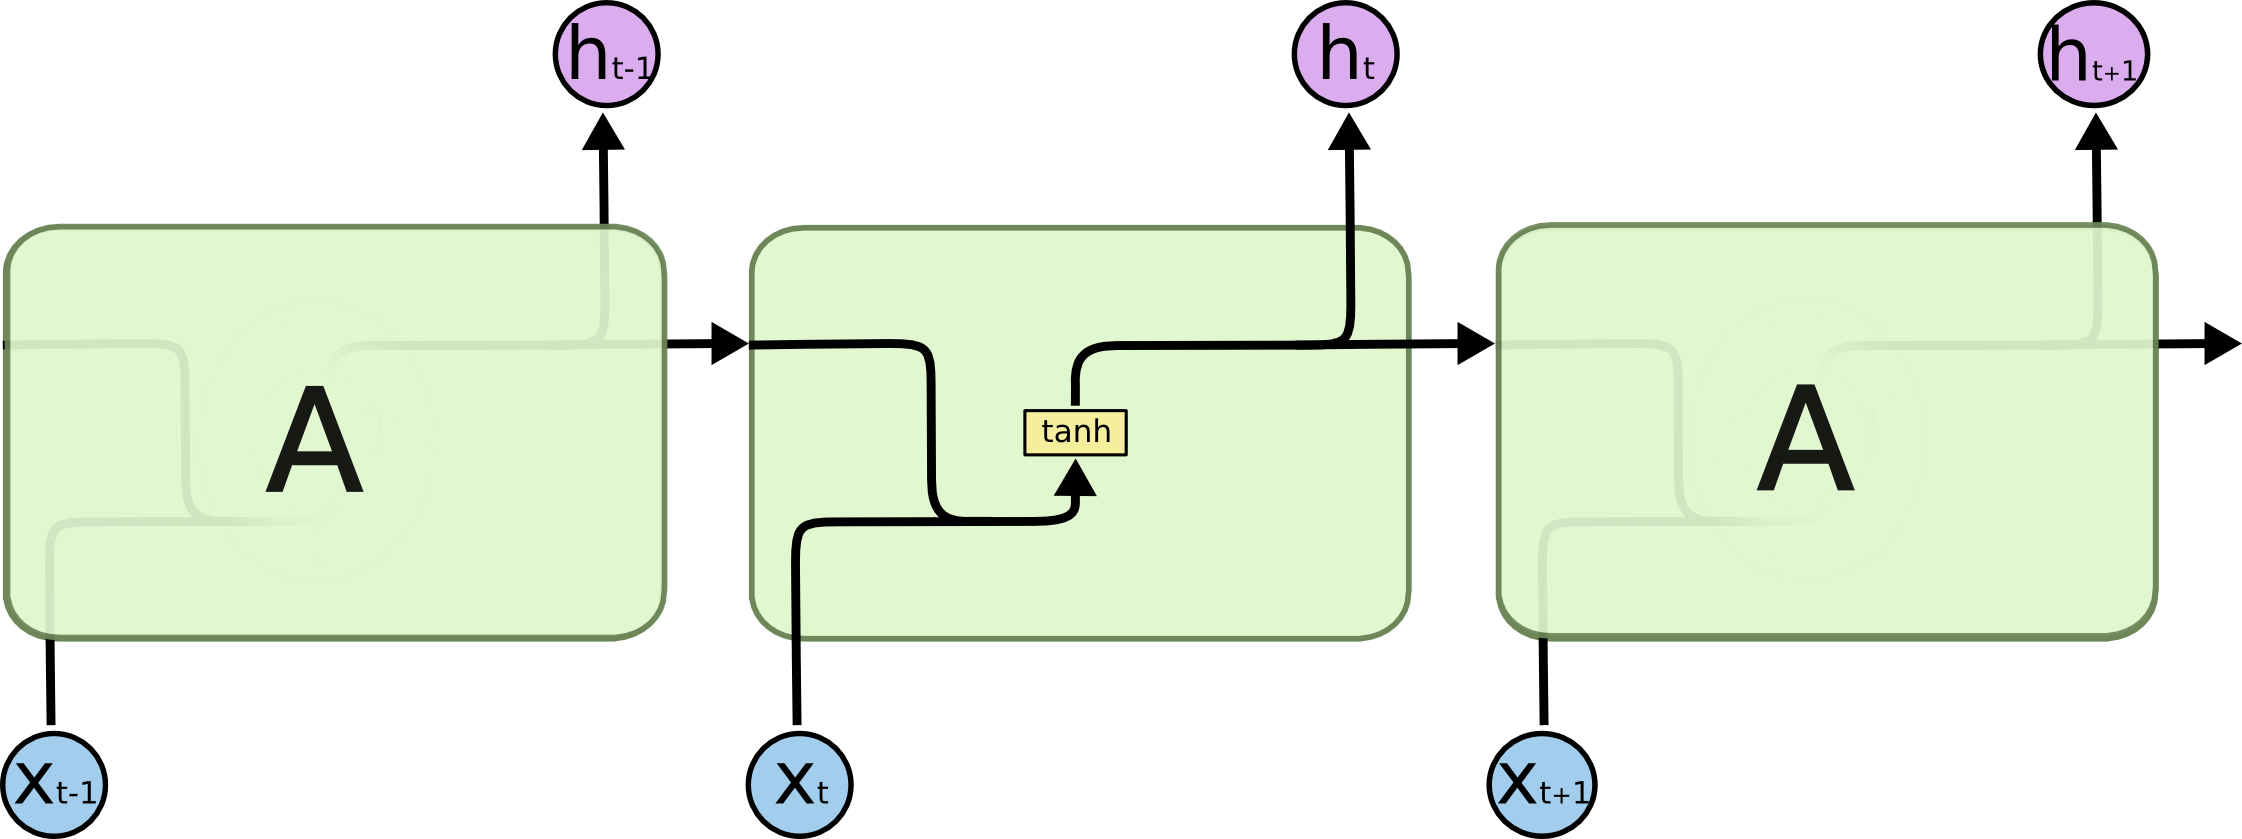
\includegraphics[width=\textwidth]{img/LSTM3-SimpleRNN.png}
  \caption{An unit in a recursive neural network, unrolled over time. Source: \url{http://colah.github.io/posts/2015-08-Understanding-LSTMs/}}
\label{fig:RNN}
\end{figure}


\subsubsection*{Long Short-Term Memory (LSTM) Networks}
\label{subs:Long Short-Term Memory (LSTM) Networks}


While Recurrent Neural Networks can model longer dependencies than e.g. Hidden Markov Models in theory, long-term dependencies are often still difficult to learn for such models. The reason is that when training the network with back-propagation, the gradient error signals are multiplied over many time steps, weakening the signal. This weakness is known as the \emph{vanishing gradient problem} which was formalized and studied in depth by~\cite{Hochreiter:1991aa}. The opposite effect is known as \emph{exploding gradients} where the gradient signal is so large that learning can diverge. Based on these insights~\cite{Hochreiter:1997aa} then introduced a new recurrent network design specifically to overcome this shortcoming.
This network architecture is called Long-Term Short Memory Network (LSTM) and has seen tremendous interest recently due to its effectiveness for learning sequential and temporal structure. In many popular application domains in machine learning it achieves state-of-the-art results, including sequence to sequence language translation, handwriting recognition and generative sequence modeling (see e.g.~\cite{Greff:2015aa} where popular variants of the architecture are compared and applied to a set of problems). Similar to the developments in \gls{Deep Learning}, much of the recent successes have just recently been made possible with technological advancement of concurrent computational hardware, specifically \glspl{GPU}, as recurrent neural networks are very expensive to train in terms of computational resources due to their complexity.

\begin{figure}[h]
  \centering
  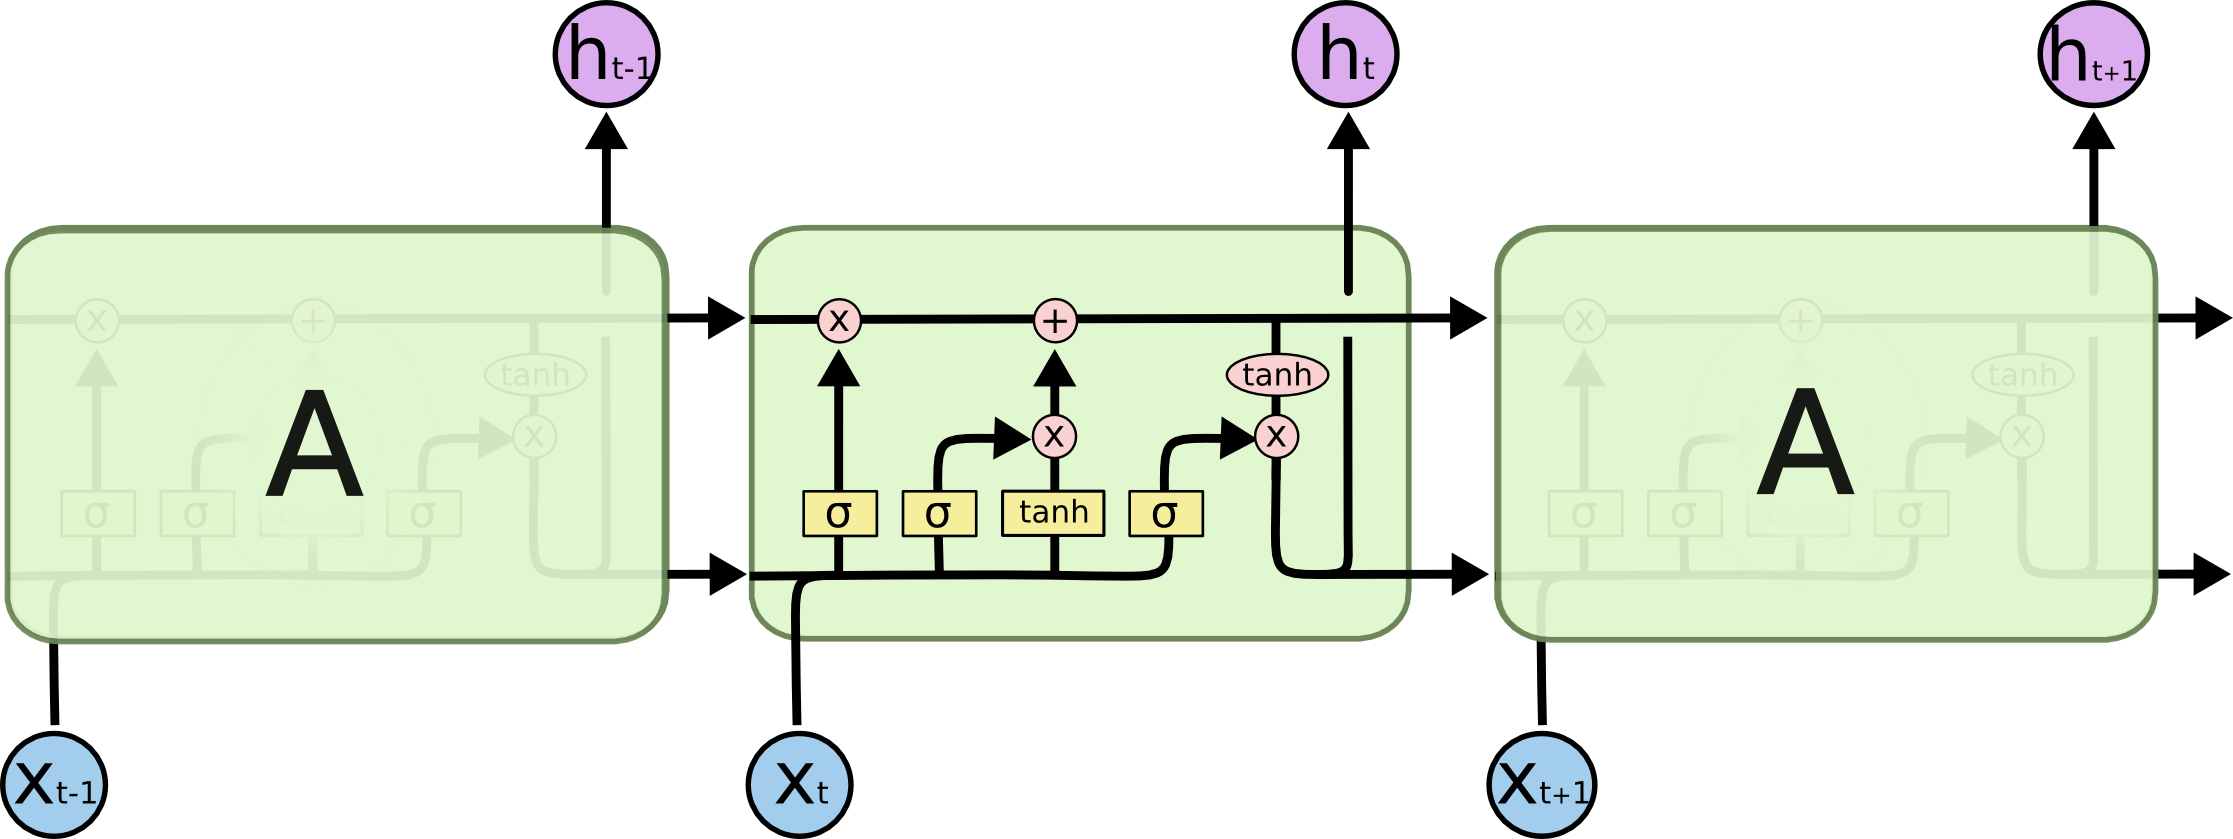
\includegraphics[width=\textwidth]{img/LSTM3-chain.png}
  \caption{An unrolled LSTM node, showing the architecture. Source: \url{http://colah.github.io/posts/2015-08-Understanding-LSTMs/}}
  \label{fig:LSTM}
\end{figure}

The specific architecture can be seen in Figure~\ref{fig:LSTM}, again unrolled over time as above. A node in an LSTM network introduces a few modifications to a standard cell in a traditional \gls{RNN}. The current cell state is passed through to the next time step by default. This signal can be intercepted by a number of so-called \emph{gates} depending on the previous cell state, the previous cell output and the current data input.
The first of such interactions is the \emph{forget gate} that was in fact a later addition to the model introduced in~\cite{Gers:1999aa} but is now considered part of the standard LSTM model. The forget gate is a sigmoid function receiving the previous cell output and the current data input and can influence how much of the cell state is kept or ``forgot''. Next the \emph{input gate} with a sigmoid function determines which values will be updated in the cell and another $\tanh$ activation node selects candidates for the update based on the previous cell output, replacing the current cell state. Lastly the cell outputs the updated cell state and the cell output based on what the input gate let through.

As mentioned early there are many variants, extensions and simplifications of this model. The previously mentioned study by~\cite{Greff:2015aa} offers a good overview as well as a comparative study by~\cite{Zaremba:2015aa}. For a comprehensive introduction to Recurrent Neural Networks the reader shall be referred to~\cite{Graves:2012aa}.

\subsection{Evaluation Metrics}
\label{sub:Evaluation Metrics}

In this section the basics of evaluating classification models for the given problem will be laid out. First the different evaluation schemes and their advantages or disadvantages are explained in the dichotomous case where only one class is to be predicted in terms of being active or not. Then these are generalized to the multi-label case where $K$ mutually exclusive classes are given. The last section extends this concept again towards so-called multi-label multi-output classification where several output labels can be predicted at the same time.

\subsubsection*{Binary Classification}
\label{subs:Binary Classification}

In the binary case of classification we are given a single class $k$ and a set of labelled data points $\mathcal{D} = \{ (x_1, y_1), (x_2, y_2), \ldots, (x_n, y_n) \}$ where targets $y_i \in \{0, 1\}$ encode whether a data point $x_i$ belongs the class $c$ or not. The task is then to achieve correct classification of new data points without knowing the true label via a model function or predictor $f(\cdot)$.

To evaluate such a predictor it is useful to present the results in form of a contingency table as shown in table Table~\ref{table:contingency-table-2}, because it gives valuable insights about the performance of the prediction. The table shows the proportion of data points that belong to the class (RP) or not (RN) and were predicted correctly (TP) or incorrectly (FN), as well as the number of data samples that do not belong to the class (RN) and were falsely predicted to be in the class (FP) or correctly predicted to not be in the class (TN), and the same proportions for the positively (PP) and negatively (PN) predicted cases with respect to the true assignments to the data. N refers to the total amount of data points.

\begin{table}[h]
  \begin{center}
    \begin{tabular}{r | c c }
      & Real Positives (RP) & Real Negatives (RN) \\
      \hline
      Predicted Positives (PP) & True Positives (TP) & False Positives (FP) \\
      Predicted Negatives (PN) & False Negatives (FN) & True Negatives (TN) \\
    \end{tabular}
  \caption{Contingency table for binary classification}
\label{table:contingency-table-2}
  \end{center}
\end{table}

\paragraph{Accuracy}
\label{par:Accuracy}

An intuitive choice towards classification is to simply ask which data points were correctly classified to belong to the class or not. In terms of the contingency table above the ratio of $(\text{TP} + \text{FP}) / (\text{N})$, commonly referred to as the ``accuracy'' of the classifier.

This choice can give a good intuition and it does capture the effectiveness on both true positives as well as true negatives, but it is strongly influenced by bias of the true and predicted class distribution (known as prevalence RP/N and label bias) as pointed out by~\cite{Powers:2011aa}. For example given a population of 900 positive and 100 negative examples, a predictor that simply always chooses a positive assignment can achieve accuracy of 90\% while it obviously is not a great predictor.

\textquote{There is a good reason why accuracy is not an appropriate measure for information retrieval problems. In almost all circumstances, the data is extremely skewed: normally over 99.9\% of the documents are in the nonrelevant category. A system tuned to maximize accuracy can appear to perform well by simply deeming all documents nonrelevant to all queries. Even if the system is quite good, trying to label some documents as relevant will almost always lead to a high rate of false positives. However, labeling all documents as nonrelevant is completely unsatisfying to an information retrieval system user. }\cite[Chapter 8.3, p.~155]{Manning:2008aa}

\paragraph{Precision, Recall and F1 Score}
\label{par:Precision, Recall and F1 Score}

In the field of Information Retrieval it is common practice to measure the effectiveness of a predictive system in terms of its precision and recall.
The precision of such system is \textquote{the proportion of retrieved material that is actually relevant} whereas the recall measures \textquote{proportion of relevant material actually retrieved in answer to a search request}~\cite{Rijsbergen:1979aa}. Formally these two measures are defined as:

\begin{equation}
    \text{Precision} = \frac{\text{TP}}{\text{TP} + \text{FP}}
\end{equation}
\begin{equation}
    \text{Recall} = \frac{\text{TP}}{\text{TP} + \text{FN}}
\end{equation}


As both, high precision and recall, are important for an robust information retrieval system they are typically combined into a single measure such as the F-measure, also referred to as F-score. The F-score is the weighted harmonic mean between precision and recall, derived from the measure of effectiveness proposed in~\cite{Rijsbergen:1979aa}. The most common form is the $F_1$ score  where precision and recall are assigned equal weight:
\begin{equation}
  \label{f1measure}
  F_1 = 2 \cdot \frac{\text{Precision} \cdot \text{Recall}}{\text{Precision} + \text{Recall}}
\end{equation}

The $F_1$ score has the advantage of its intuitive interpretability as both precision and recall are well understood measures and, analogous to recall, precision and accuracy, as it lives in the range $[0,1]$, giving a single number that can express the effectiveness of the system in terms of percentage.

The F1 score is widely used in the field of Machine Learning and Data Mining and thus it is an important measure to consider to compare results to outcomes of prior publications by others.
It is however important to point out that any version of the F-measure is a biased score as it \textquote{ignores TN which can vary freely without affecting the statistic}~\cite{Powers:2011aa}. This can affect the evaluation of a classifier when the class distribution is skewed (prevalence) or the classifier develops a bias towards certain classes (label bias), motivating the use of unbiased measures in these cases, such as the ones described next.

\paragraph{Informedness, Markedness and Matthews Correlation Coefficient}
\label{par:Informedness, Markedness and Matthews Correlation Coefficient}

\cite{Powers:2011aa} introduces unbiased analogue measures to Recall and Precision, called ``Informedness'' and ``Markedness'' respectively. As~\cite{Powers:2011aa} lays out, \blockquote{Informedness quantifies how informed a predictor is for the specified condition, and specifies the probability that a prediction is informed in relation to the condition (versus chance).}:

\begin{equation}
  \begin{split}
  \text{Informedness} &= \text{Recall} + \text{Inverse Recall} \text{ – } 1 \\
  &=\frac{\text{TP}}{ \text{RP}} + \frac{\text{TN}}{\text{RN}} \text{ – } 1
  \end{split}
\end{equation}

Further he defines:
\blockquote{Markedness quantifies how marked a condition is for the specified predictor, and specifies the probability that a condition is marked by the predictor (versus chance).}

\begin{equation}
  \begin{split}
  \text{Markedness} &= \text{Precision} + \text{Inverse Precision} \text{ – } 1\\
  &=\frac{\text{TP}}{ \text{PP}} + \frac{\text{TN}}{\text{PN}} \text{ – } 1
  \end{split}
\end{equation}

Based on Informedness and Markedness we can then see that \emph{Matthews Correlation Coefficient} $r_{G}$, first proposed by~\cite{Matthews:1975aa}, is a score that balances these two measures:

\begin{equation}
  \begin{split}
  r_{G} &= \pm \sqrt{\text{Informedness} \cdot \text{Markedness}} \\
  &= \frac{(\text{TP} \cdot \text{TN} - \text{FP} \cdot \text{FN})}{(\text{TP} + \text{FN})(\text{FP} + \text{TN})(\text{TP} + \text{FP})(\text{FN} + \text{TN})}
\end{split}
\end{equation}

Matthews Correlation Coefficient can thus be used as unbiased alternative to the F-measure and offers a similar ease of interpretability as it ranges from -1 to 1, the former indicating a negative correlation or adverse estimation and the latter  indicating a perfect prediction, while a coefficient of 0 reflects chance.

\paragraph{Cross-Entropy}
\label{par:Cross-Entropy}

Another common way to evaluate classifiers is the \emph{cross-entropy} loss function:

\begin{equation}
  \mathbb{H}(p,q) = - \sum_n^N p_n \log q_n
\end{equation}

where $p$ and $q$ are discrete probability distributions. The \emph{cross-entropy} can be derived from the \emph{KL-divergence} as in~\cite[Chapter 2.8.2, p.~57]{Murphy:2012aa}:

\begin{equation}
  \begin{split}
  \mathbb{KL}(p,q) &= \sum_n^N p_n \log \frac{p_n}{q_n} \\
  &= \sum_n^N p_n \log p_n - \sum_n^N p_n \log q_n \\
  &= - \mathbb{H}(p) + \mathbb{H}(p,q)
\end{split}
\end{equation}

where $\mathbb{H}(p)$ is the regular entropy, i.e.\ the lower bound on the number of bits needed to transmit the state of a random variable (as in~\cite{Shannon:2001aa}), and $\mathbb{H}(p,q)$ is the cross-entropy, i.e. \textquote{the average number of bits needed to encode data coming from a source distribution $p$ when we use model $q$ to define our codebook}~\cite[Chapter 2.8.2, p.~57]{Murphy:2012aa}.

In the case of binary classification we can rewrite the cross-entropy into the following error or loss function of the learned weight vector:

\begin{equation}
  E(\mathbf{w}) =  -\log p(\mathbf{T} \mid \mathbf{w}) = - \sum_{n=1}^N {t_n \log y_n + (1 - t_n) \log (1 - y_n)}
\end{equation}

where $y_n$ denotes $y(x_n, \mathbf{w})$, the predicted output for datapoint $x_n$, $t_n$ denotes the $n$-th true label and $\mathbf{w}$ denotes the trained weight vector of the model, as in~\cite[Chapter 4.3.2, p.~205 ]{Bishop:2006aa}. This form is also known as the \emph{log loss} and it is commonly used with generalized linear models and \glspl{NN} (see e.g.~\cite[Chapter 4.3.2, p.~205 ]{Bishop:2006aa} and~\cite[Chapter 10.7, p.~251 ]{Alpaydin:2014aa}).

Thus, cross-entropy is a measure which is well-motivated from a information-theoretic perspective. On the downside it does not have an upper bound which makes it hard to interpret, as compared other scores that fall into $[0, 1]$ or similar intervals.

\subsubsection*{Multi-class Classification}
\label{subs:Multi-class Classification}

Multi-class classification refers to a generalization of the binary case where we aim to predict for each datapoint $wowx_i$ one of $K$ labels for the classes at hand. The target space $\mathcal{Y}$ can be represented with each $y_i \in \{ 0,1 \}^k$, known as \emph{one-hot encoding}, where each target is $c$-dimensional vector. Alternatively we can encode the targets as categorical variables $y_i \in {c_1, c_2, \ldots, c_k}$. The contingency table from the binary case can be extended as in table~\ref{table:contingency-table-k}, which is then commonly known as
\gls{Confusion Matrix} or \gls{Error Matrix}.

\begin{center}
  \begin{table}[h]
  \begin{tabular}{r | c c c c }
    & Real Class 1 & Real Class 2 & \ldots & Real Class $k$ \\
    \hline
    Predicted Class 1    & \ldots & \ldots & & \ldots \\
    Predicted Class 2    & \ldots & \ldots & & \ldots \\
    \ldots               & & & & \\
    Predicted Class $k$  & \ldots & \ldots & & \ldots \\
  \end{tabular}
  \caption{Contingency table for $k$ classes, also referred to as Confusion Matrix}
\label{table:contingency-table-k}
\end{table}
\end{center}

\paragraph{Averaging for Multi-class Recall, Precision and F1-Score}
\label{par:Averaging for Multi-class Recall, Precision and F1-Score}

By definition, Recall, Precision and thus also the F-measure are defined for the dichotomous classification case, however they can be extended towards multiple classes by averaging. Two common methods are described in~\cite[Chapter 13.6, p.~280]{Manning:2008aa}: \textquote{Macroaveraging computes a simple average over classes. Microaveraging pools per-document decisions across classes, and then computes an effectiveness measure on the pooled contingency table.}
It is important to note that \textquote{macroaveraging gives equal weight to each class, whereas microaveraging gives equal weight to each per-document classification decision. Because the F1 measure ignores true negatives and its magnitude is mostly determined by the number of true positives, large classes dominate small classes in microaveraging.}~\cite[Chapter 13.6, p.~280]{Manning:2008aa}. Formally these averaging schemes can be defined as follows, with R denoting the Recall and P the Precision.

\begin{equation}
  \text{R}_{\text{micro}} = \frac{\sum_{k=1}^K \text{TP}_k }{ \sum_{k=1}^K \text{TP}_k + \text{FN}_k } \qquad
  \text{R}_{\text{macro}} = \frac{\sum_{k=1}^K \text{R}_k }{ K }
\end{equation}
\begin{equation}
  \text{P}_{\text{micro}} = \frac{\sum_{k=1}^K \text{TP}_k }{ \sum_{k=1}^K \text{TP}_k + \text{FP}_k } \qquad
  \text{P}_{\text{macro}} = \frac{\sum_{k=1}^K \text{P}_k }{ K }
\end{equation}

And respectively:

\begin{equation}
  \text{F}_{1 \text{micro}} = 2 \cdot \frac{\text{P}_{\text{micro}} \cdot \text{R}_{\text{micro}} }{\text{P}_{\text{micro}} + \text{R}_{\text{micro}} } \qquad
  \text{F}_{1 \text{macro}} = 2 \cdot \frac{\text{P}_{\text{macro}} \cdot \text{R}_{\text{macro}} }{\text{P}_{\text{macro}} + \text{R}_{\text{macro}} }
\end{equation}

\paragraph{Matthews Correlation Coefficient for K classes}
\label{par:Matthews Correlation Coefficient for K classes}

\cite{Gorodkin:2004aa} introduced a way to extend Matthews Correlation Coefficient to the multi-class case using a generalization of Pearson’s Correlation Coefficient. The coefficient is then defined as:

\begin{equation}
  R_k  = \frac{\text{COV}(X, Y)}{\sqrt{\text{COV}(X, X) \ \text{COV}(Y, Y)}}
\end{equation}

Where $\text{COV}$ is the covariance function:

\begin{align}
  \text{COV}(X, Y) &= \sum_{k=1}^K w_k \text{COV}(X_k, Y_k) \\
  &= \frac{1}{K} \sum_{n=1}^N \sum_{k=1}^K (X_{nk} - \overline{X_k})(Y_{nk} - \overline{Y_k})
\end{align}

Similar extensions have been proposed, such as the Confusion Entropy (CEN) as described in~\cite{Jurman:2012aa}. The article concludes:

\blockquote{Confusion Entropy [\ldots] is probably the finest measure and it shows an extremely high level of discriminancy even between very similar confusion matrices. However, this feature is not always welcomed, because it makes the interpre- tation of its value quite harder, expecially when considering sit- uations that are naturally very similar (e.g, all the cases with MCC=0). Moreover, CEN may show erratic behaviour in the binary case.

In this spirit, the Matthews Correlation Coefficient is a good compromise between reaching a reasonable discriminancy degree among different cases, and the need for the practitioner of a easily interpretable value expressing the type of misclassification associated to the chosen classifier on the given task. We showed here that there is a strong linear relation between CEN and a logarithmic function of MCC regardless of the dimension of the considered problem. Furthermore, MCC behaviour is totally consistent also for the binary case.

This given, we can suggest MCC as the best off-the-shelf evaluating tool for general purpose tasks, while more subtle measures such as CEN should be reserved for specific topic where more refined discrimination is crucial.}

Thus Matthews Correlation Coefficient is the preferred measure when possible.


\paragraph{Categorical Cross-Entropy}
\label{par:Categorical Cross-Entropy}

The \emph{cross-entropy} loss function as defined above in Section~\ref{par:Cross-Entropy} extends to the multi-class case quite naturally:

\begin{equation}
  E(\mathbf{w}_1, \ldots, \mathbf{w}_k) = -\ln p(\mathbf{T} \mid \mathbf{w}_1, \ldots, \mathbf{w}_k) = - \sum_{n=1}^N \sum_{k=1}^K t_{nk} \ln y_{nk}
\end{equation}

where $y_{nk} = y_k (\phi_n)$, and $\mathbf{T}$ is an  $N \times K$ matrix of target variables with elements $t_{nk}$ (see as in~\cite[Chapter 4.3.4, p.~209 ]{Bishop:2006aa}). This form is also referred to as \emph{multi-class log loss} and gives an aggregated loss over all classes.
